\newpage
\appendix
\appendixpage
\addappheadtotoc

\setlength{\parskip}{10pt plus 4pt minus 2pt}

\section{Testing}

Due to low performance of the YOLOv5 model, video demostration was split into two. One for testing navigation in different scenarios, the other for testing face detector.


\section{Methodology}

\subsection{Containerised development environment}

Gazebo and RViz can reach 60 FPS if they are GPU accelerated. GPU accelerated Gazebo and RViz will also start faster. These are essential for faster iteration speed. Furthermore, GPU can also significantly improve the inference speed of YOLOv5 model. However, most virtual machines do not allow pass-through GPUs, and due to their technical nature, other hardware performance is degraded, so they are not ideal tool for robotics development.

In contrast, containers can run native processess, which means processes can directly access hardwares include GPUs. Moreover, environment setup is textlised in a file named Dockerfile, and any text can be tracked by Git, which means the environment setup is quite stable, and any modification on the environment is visible.

The Above comparasion is not sufficient but gives indisputable reasons that container is much preferable than virtual machine in robotics development.

In the code submitted with this report, a folder named .devcontainer which contains Dockerfile and other container-related configurations is attached. Open the code folder by VSCode with official remote contaienr development extension, and VSCode will notify this workspace can be reopened in container. To display GUI apps inside the container, external window management server (X11 or Wayland) is necessary. Remeber to adjust two container settings to suit the host environment before building the container. One is the DISPLAY environment variable, the other is mounting tmp folder of X11. Please consult search engines for more information on the window management server and these settings.


\subsection{Spawn a MMD model in Gazebo Classic}

Anime character MMD model was downloaded from \url{https://mmd.hololive.tv/}, and coffee cup-shaped chair was downloaded from \url{https://bowlroll.net/file/64137}.

Firstly, install blender and MMD Tools addon from \url{https://github.com/UuuNyaa/blender_mmd_tools}. Using the import function of the addon to load MMD file into Blender. Next, Convert the shader node of the model to Principled BSDF by clicking the "Covert to Blender"  inside the Material block of the addon shown in Figure~\ref{fig:luna-is-dancing}. Then, using the exporting to COLLADA functionality of Blender. Open the Gazebo Classic model editor, load the COLLADA file, and finally save the model. Two files, model.config and model.sdf will generated. Organise all model files into ROS standard hierarchy. Check that the model is rendered correctly in Gazebo Classic by loading it into default empty world same as Figrue~\ref{fig:luna-in-gazebo}.

\begin{figure}[htbp]
   \centering
   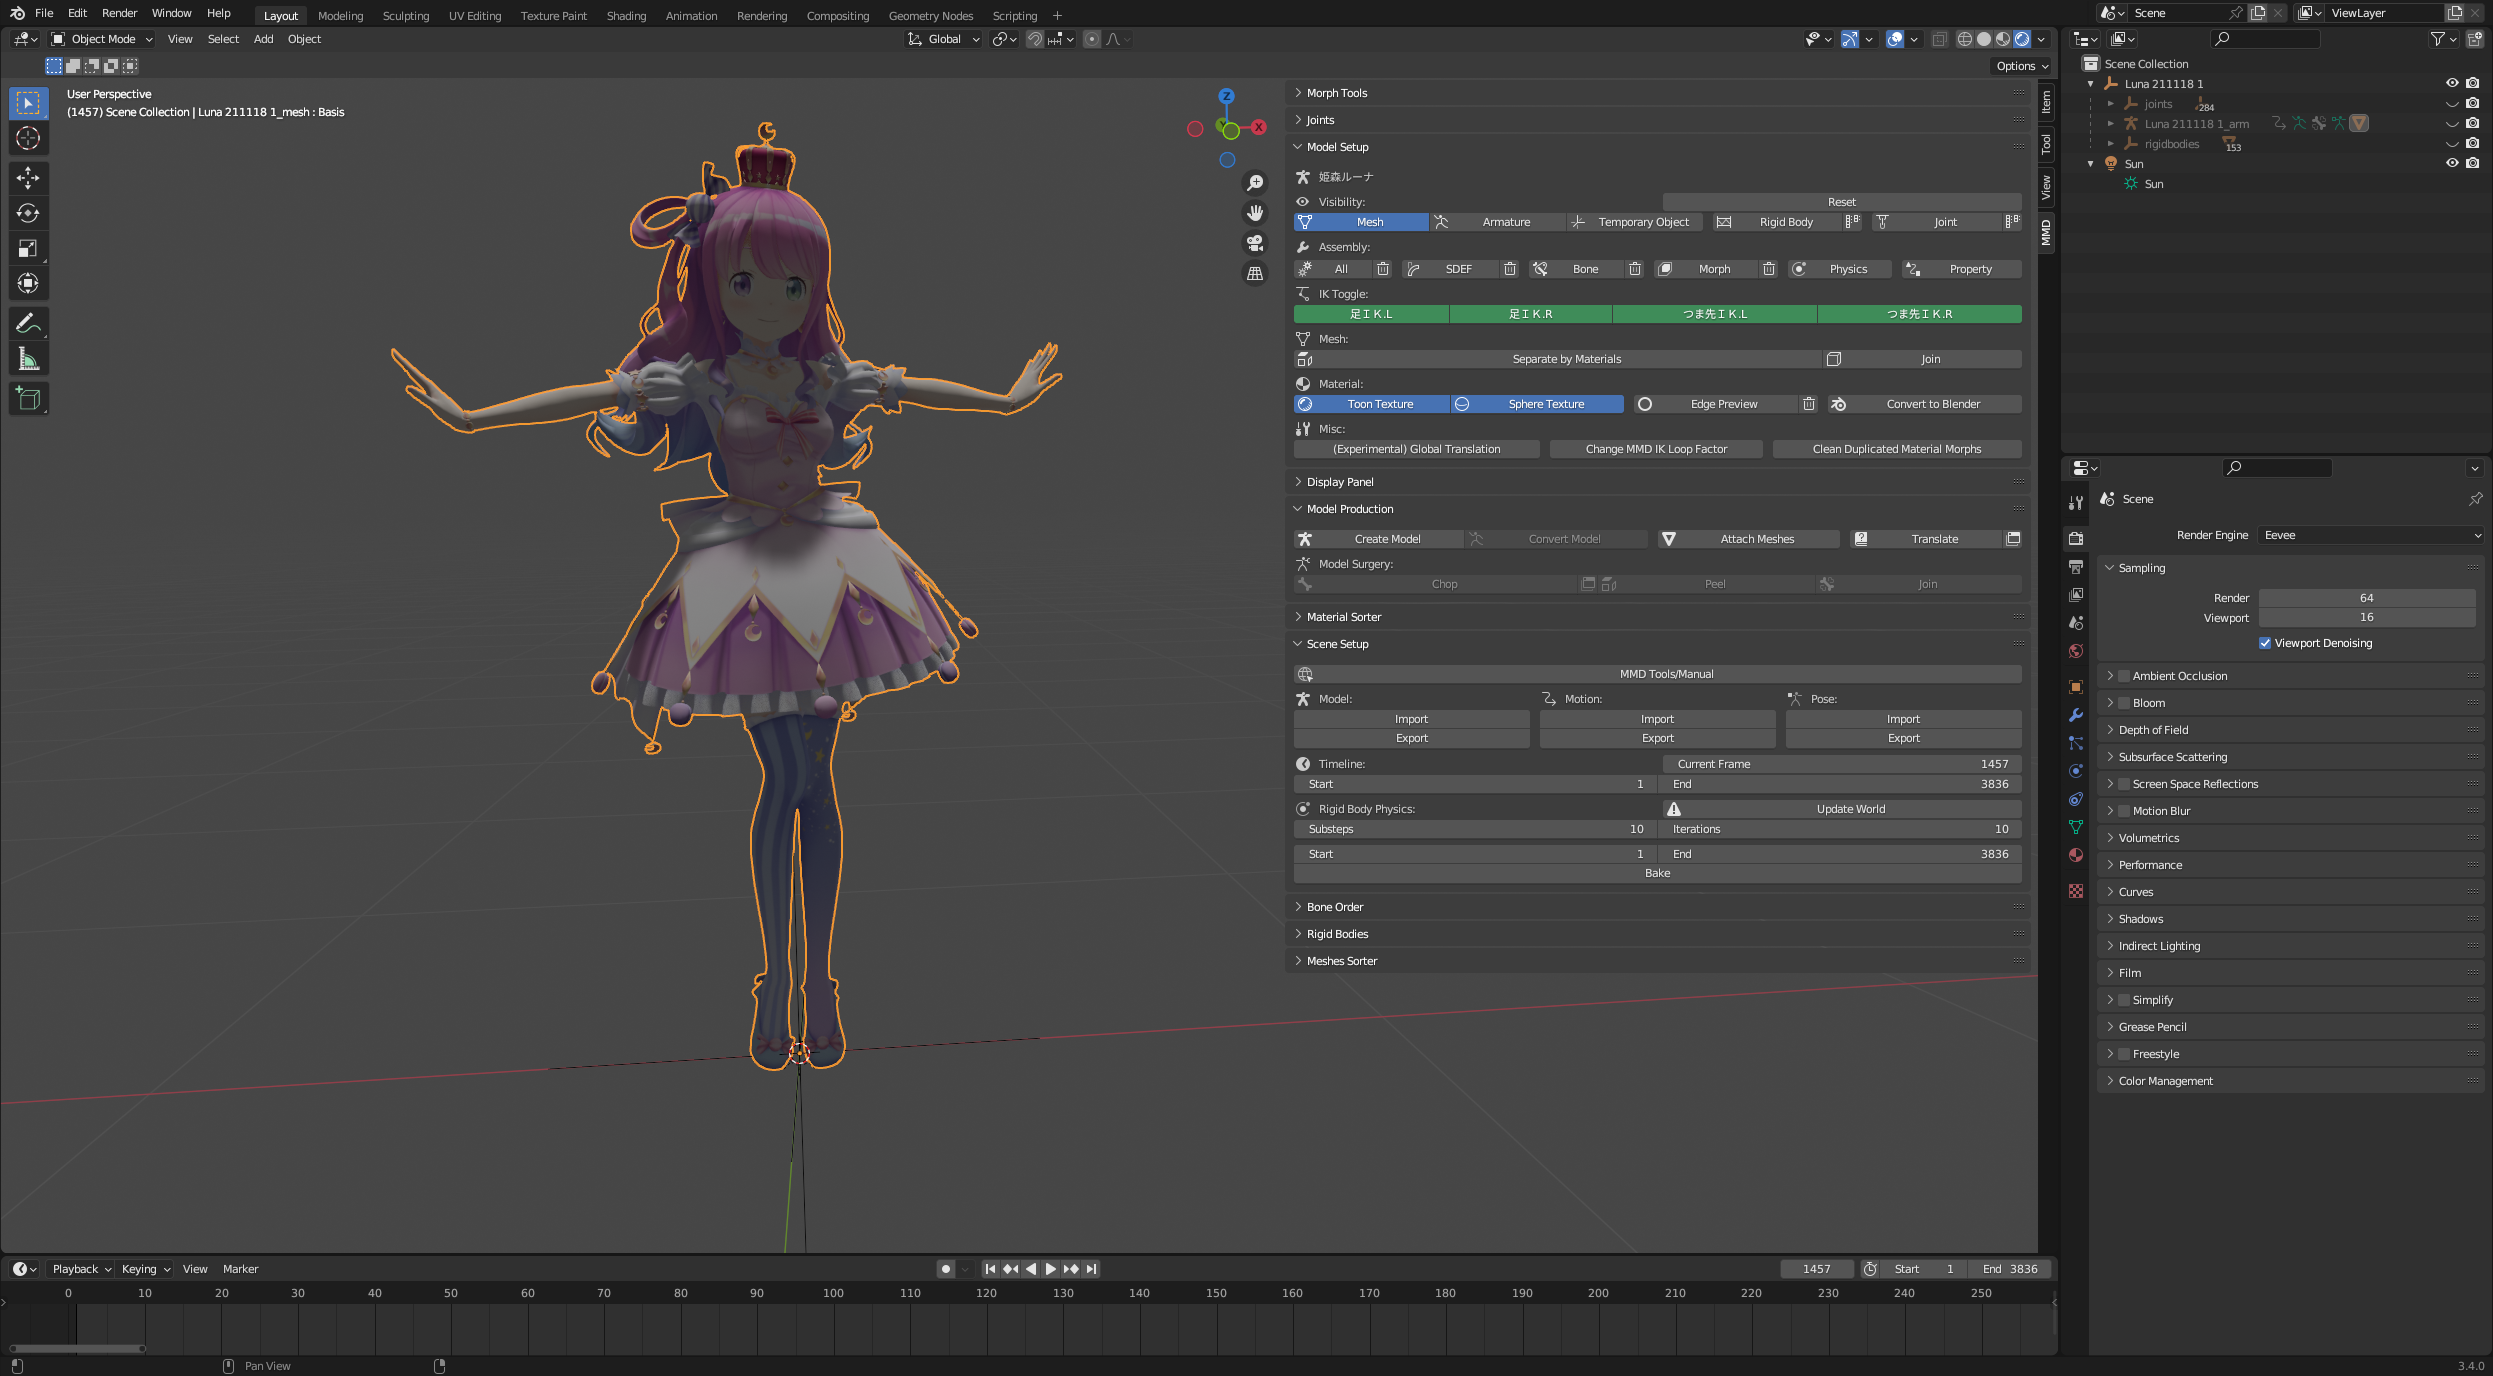
\includegraphics[width=\textwidth]{luna-is-dancing.png}
   \caption{A MMD model in Blender with MMD Tools addon tab opened}
   \label{fig:luna-is-dancing}
\end{figure}

\begin{figure}[htbp]
   \centering
   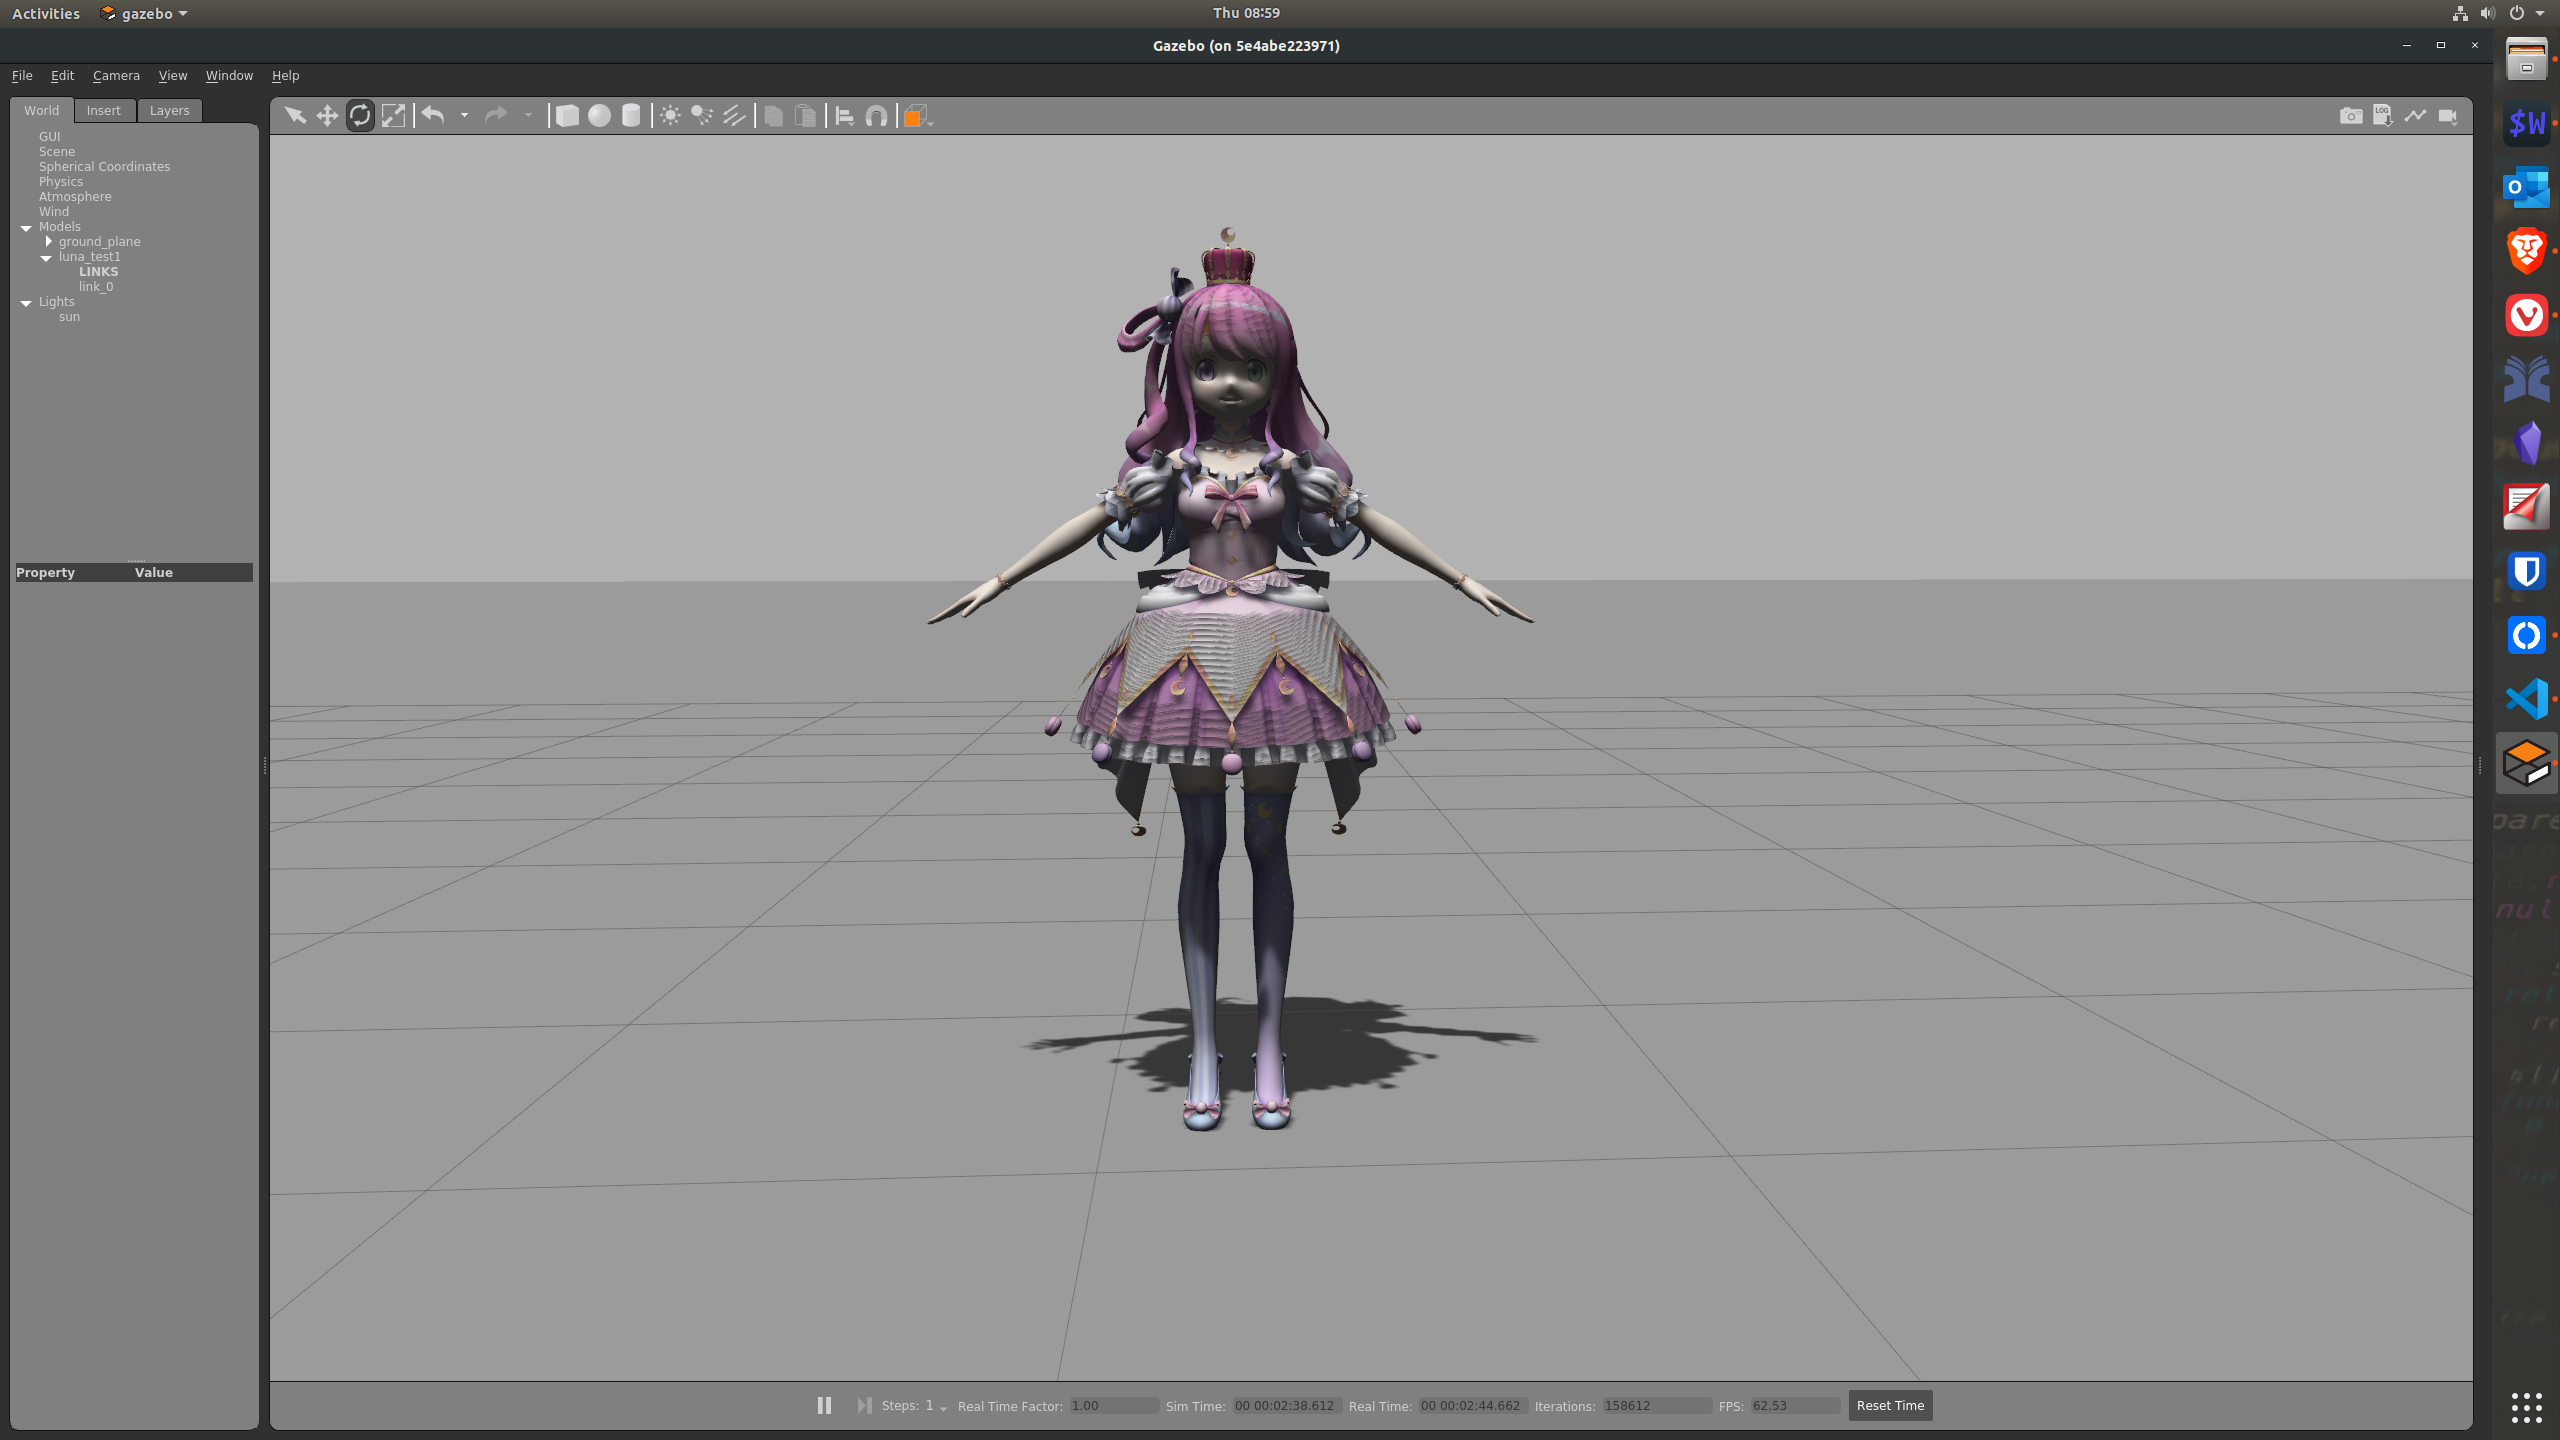
\includegraphics[width=\textwidth]{luna-in-gazebo.png}
   \caption{A MMD model in the default Gazebo Classic empty world}
   \label{fig:luna-in-gazebo}
\end{figure}


\subsection{Mapping}

Mapping was achieved by using a SLAM algorithm implemented by gmapping package with AMCL node launched. Figure~\ref{fig:gmapping} illustrates the inital state of the mapping process. Although odometry localisation can also "get the work down", AMCL gives more accurate localisation results in better map; hence the latter is prefered.

\begin{figure}[htbp]
   \centering
   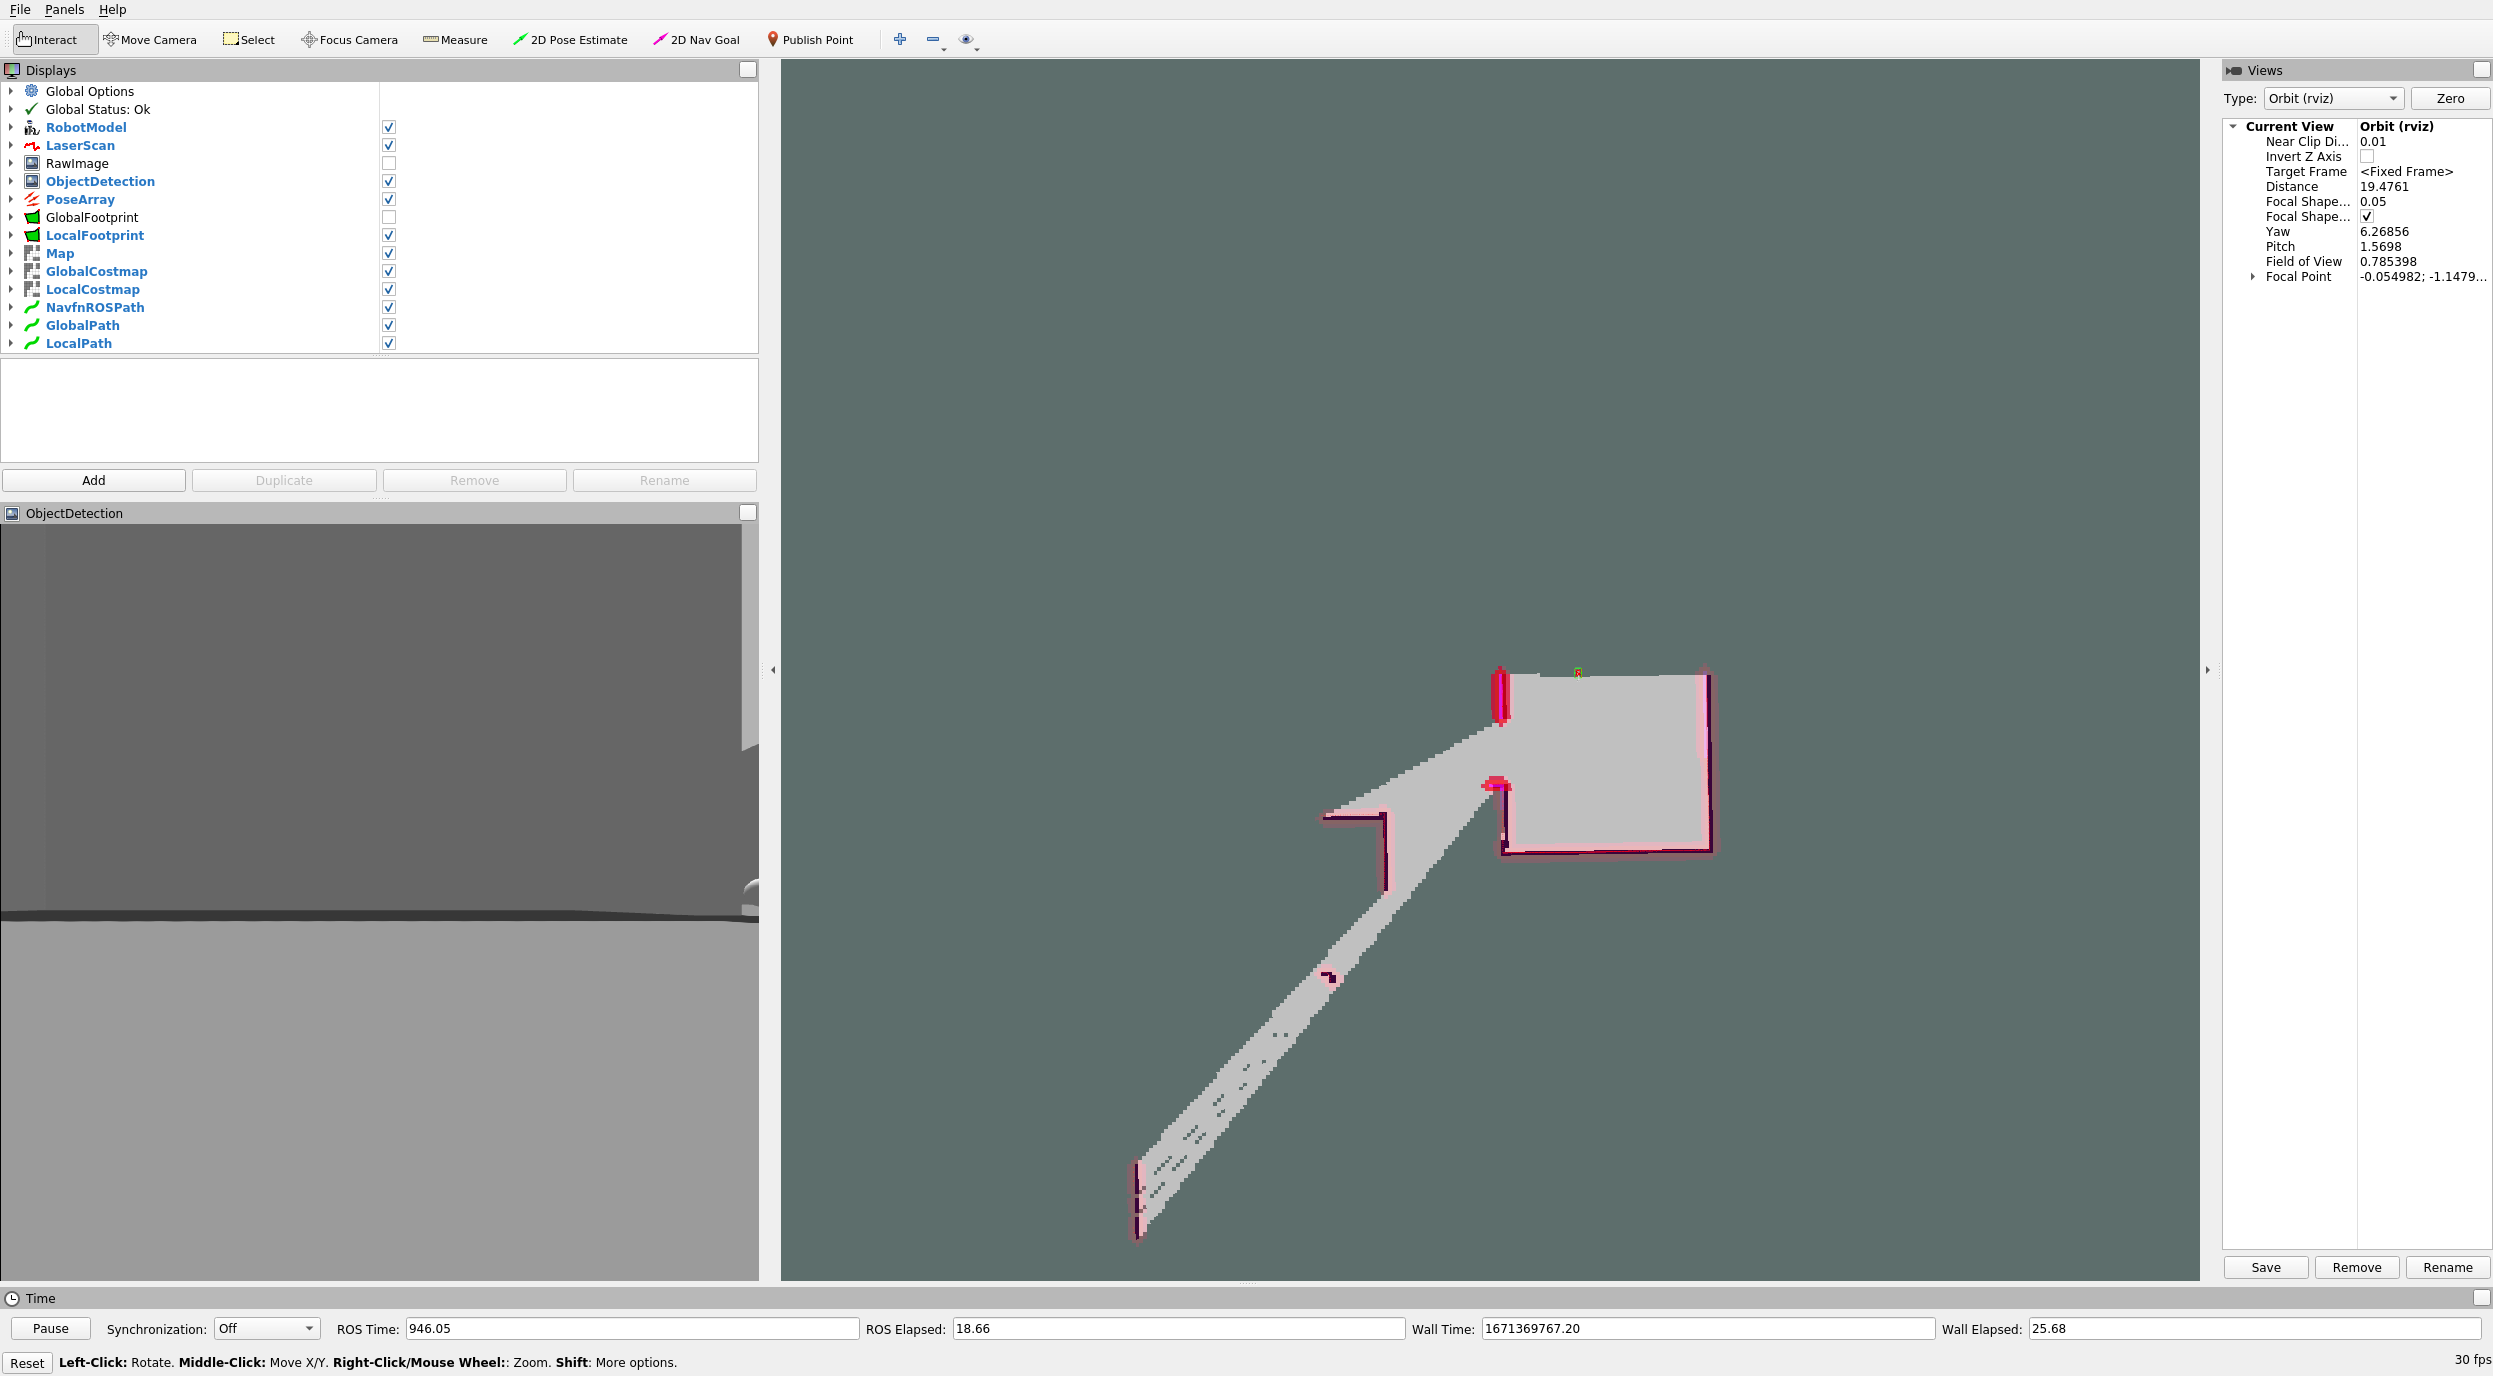
\includegraphics[width=\textwidth]{gmapping.png}
   \caption{Gmapping process visualised in RViz}
   \label{fig:gmapping}
\end{figure}

The robot can be operated manually to complete the mapping, or an algorithm such as rapidly exploring random tree (RRT) can be used to allow the robot to explore and mapping.

After mapping was completed, map saver was launched to save the map. The saved map can further be modified by drawing softwares such as GIMP to correct minor errors.


\subsection{Training YOLOv5 as face detector}

YOLOv5 \url{https://github.com/ultralytics/yolov5} is a generic object detection model based on Deep Learning. The trained model can detect multiple objects specified in training settings on an image in one inference process. After searching, a subset of WIDER FACE \url{http://shuoyang1213.me/WIDERFACE/index.html} was picked to train YOLOv5 slim architecture model as face detector. Official training guides were followed. Figure~\ref{fig:train-yolov5} shows the training process. Two NVIDIA 1080 Ti GPUs were utilised.

\begin{figure}[htbp]
   \centering
   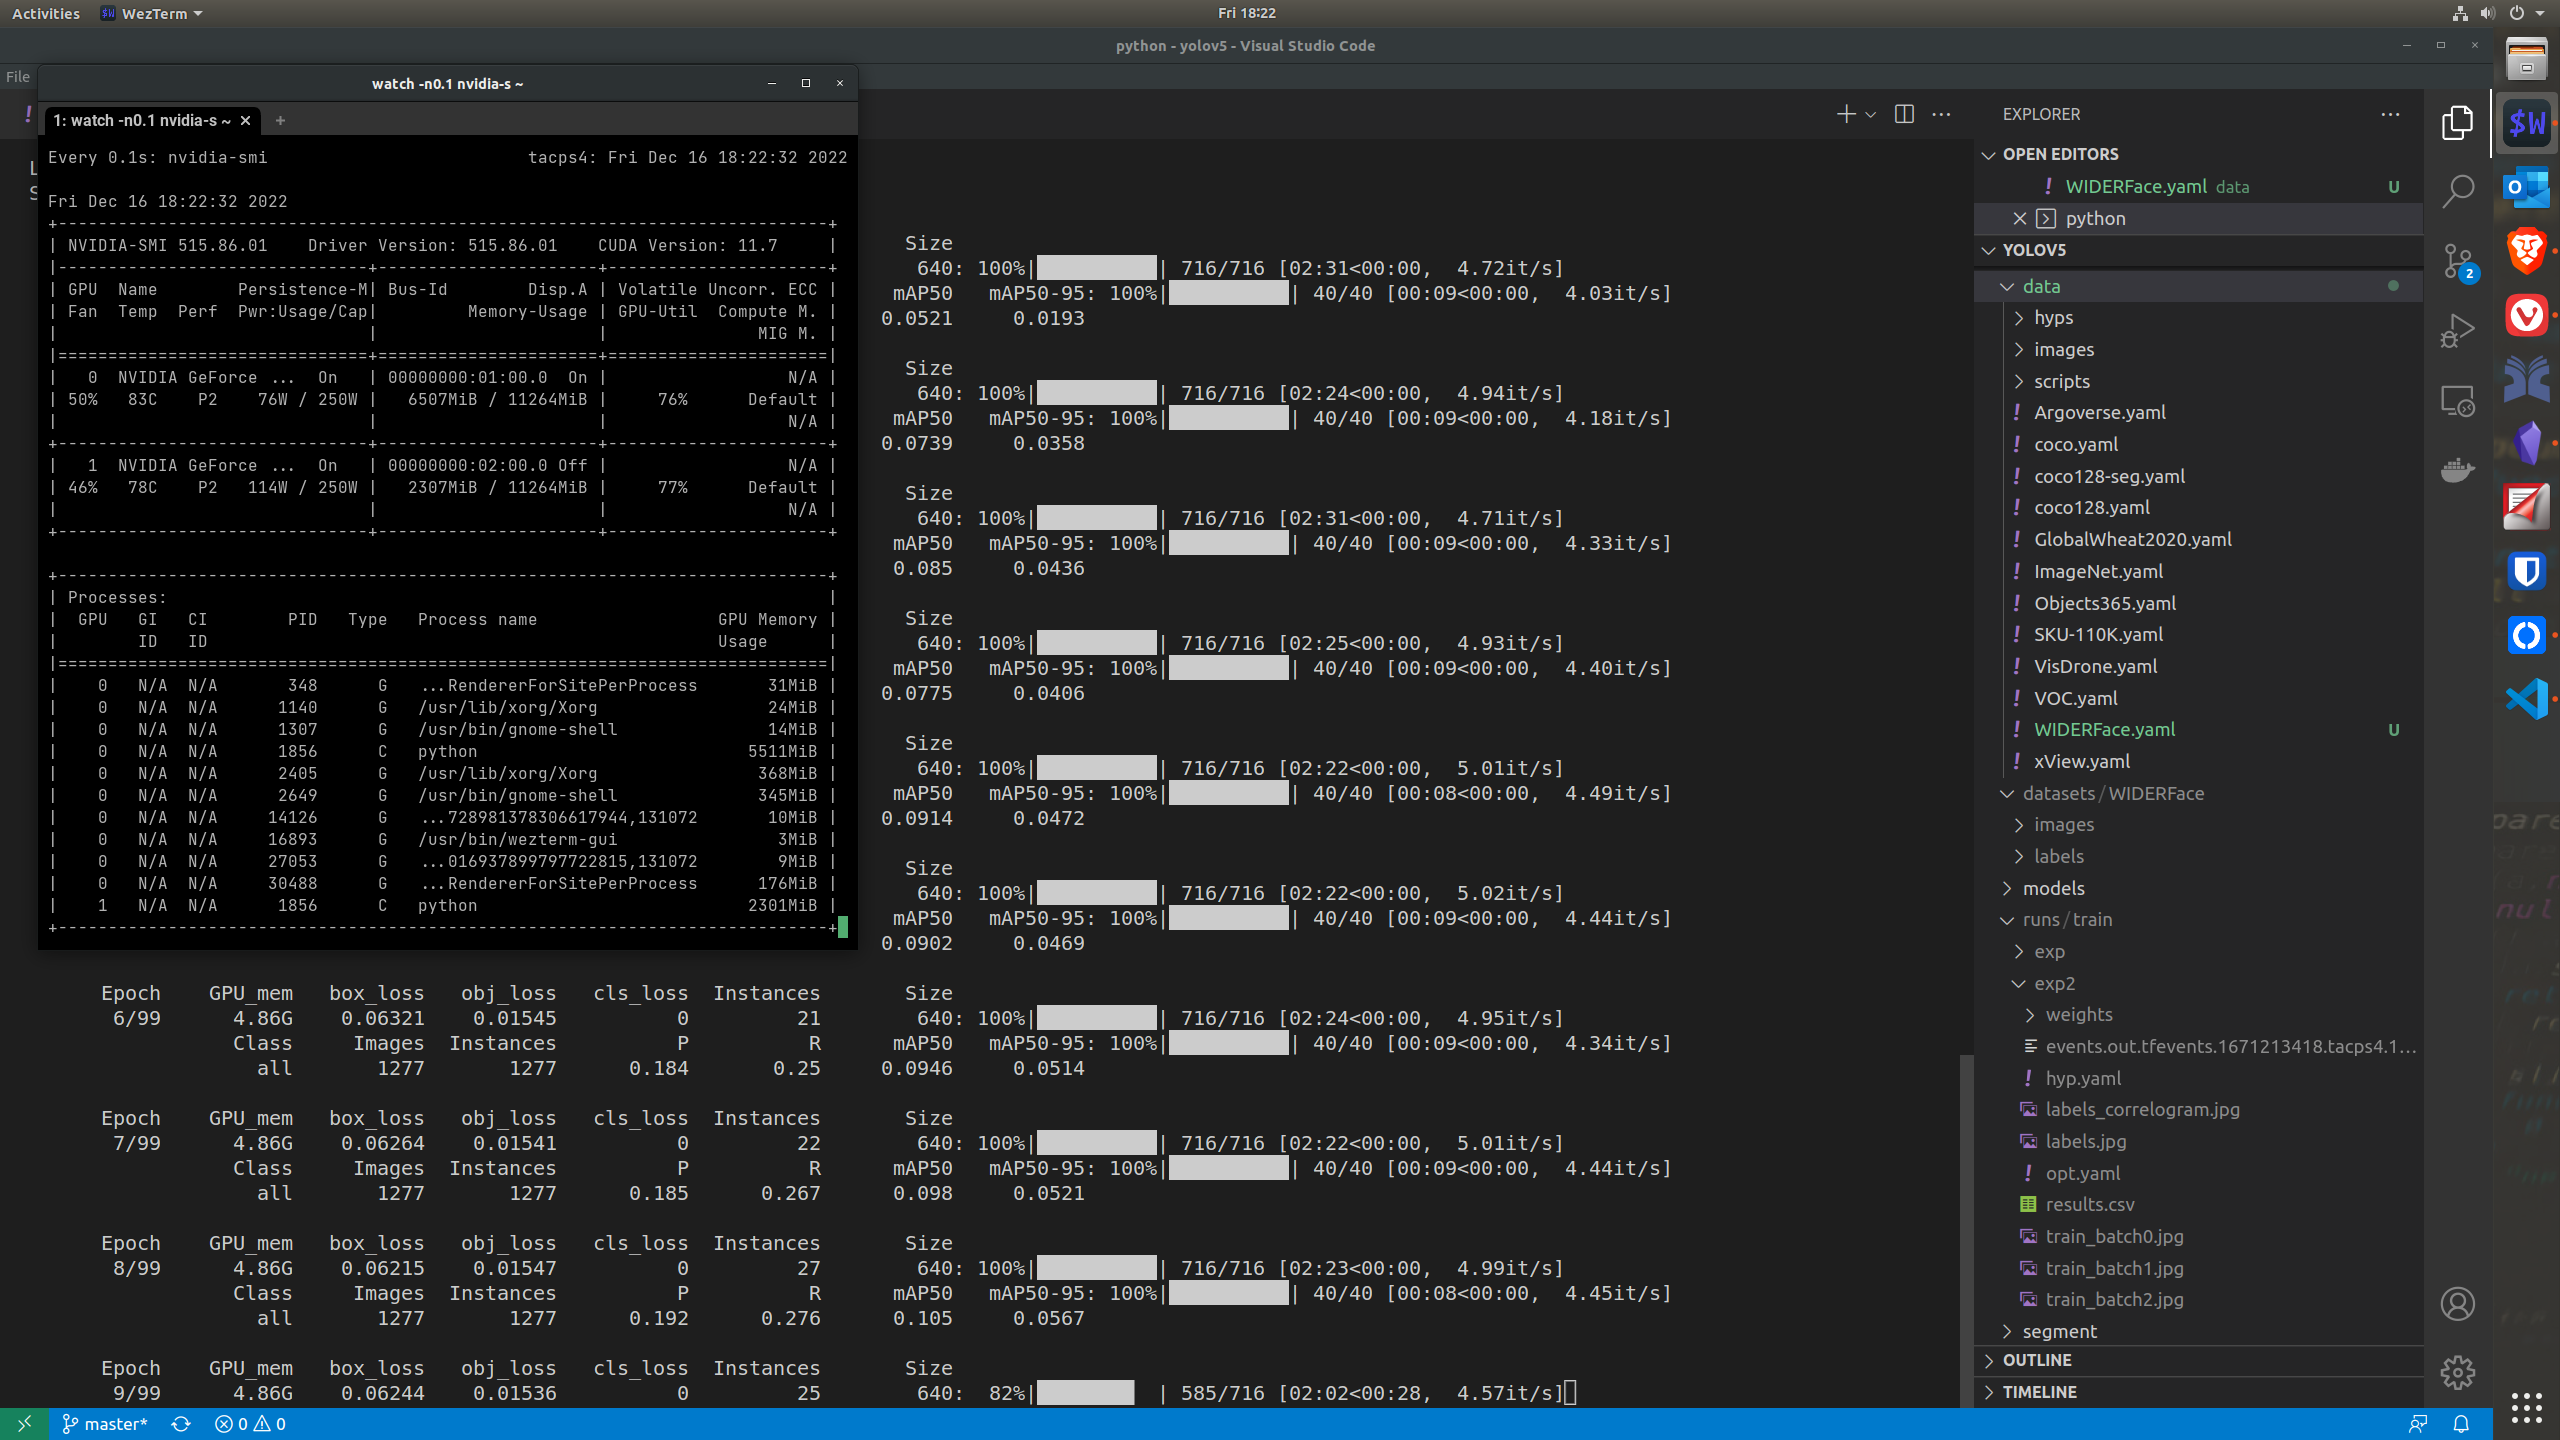
\includegraphics[width=\textwidth]{train-yolov5.png}
   \caption{Screen outputs of the YOLOv5 training process}
   \label{fig:train-yolov5}
\end{figure}

Figure~\ref{fig:real-faces-detected} is the inference result of the trained model. Notice that although the model detects all the faces in the image, the confidence is low. Normally, confidence value between 0.8 to 0.98 is expected. Low confidence indicates this model is not good enough, may be because the data are not enough since it is a very small subset (1.5G) of the original dataset (25G).

\begin{figure}[htbp]
   \centering
   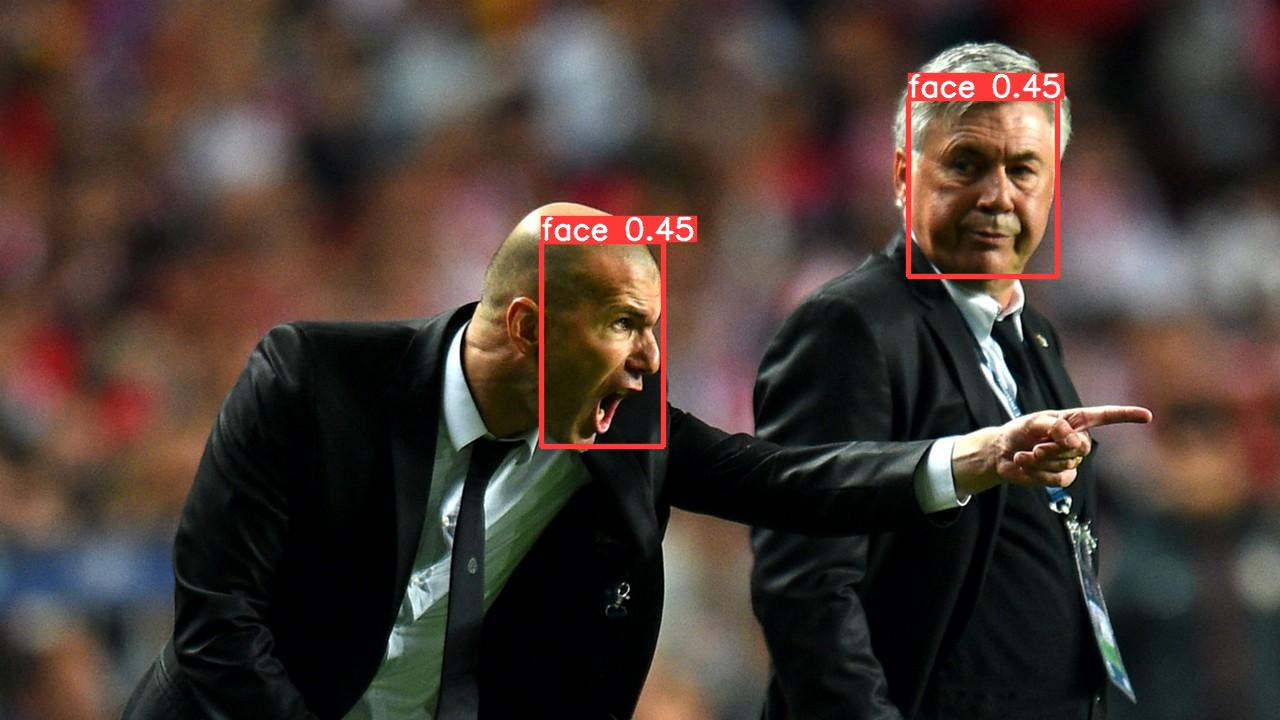
\includegraphics[width=\textwidth]{real-faces-detected.jpg}
   \caption{Real faces are detected but with low confidence}
   \label{fig:real-faces-detected}
\end{figure}

Furthermore, the model cannot detect anime faces as shown in Figure~\ref{fig:cannot-detect-anime-faces}. This may be due to the fact that there are only real faces in the dataset.

\begin{figure}[htbp]
   \centering
   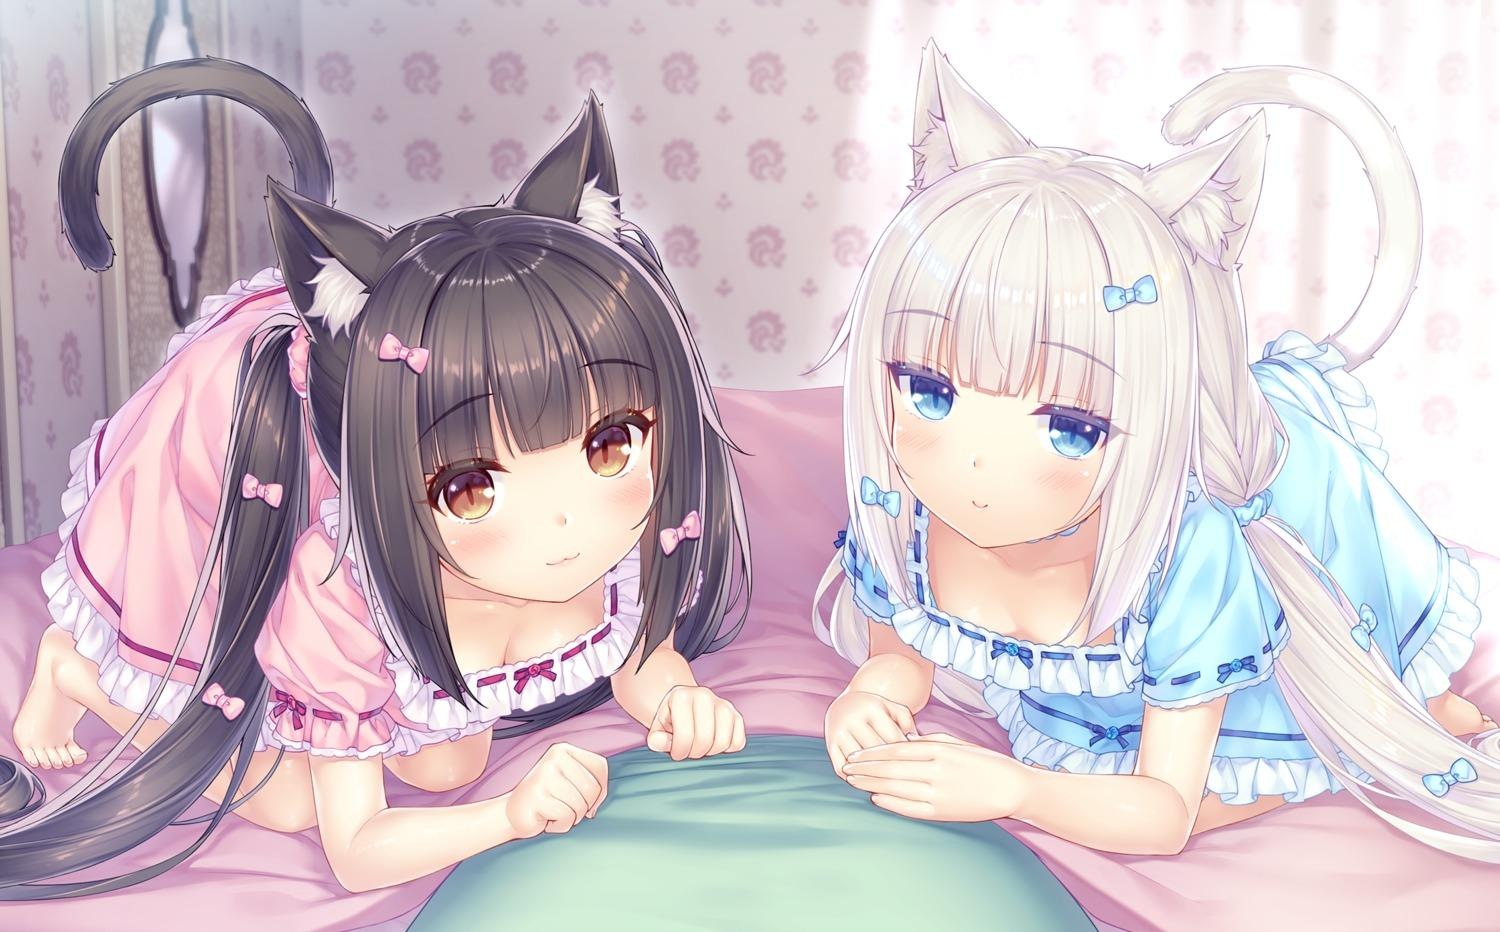
\includegraphics[width=\textwidth]{cannot-detect-anime-faces.jpg}
   \caption{Anime faces cannot be detected}
   \label{fig:cannot-detect-anime-faces}
\end{figure}


\section{Abondaned attempts due to limited time budget}

\subsection{Enlarging the tiny robot}

The tiny robot was enlarged as shown in Figure~\ref{fig:enlarged-robot} for better camera viewing point. However, the enlarged robot moves much slower than the tiny version.

\begin{figure}[htbp]
   \centering
   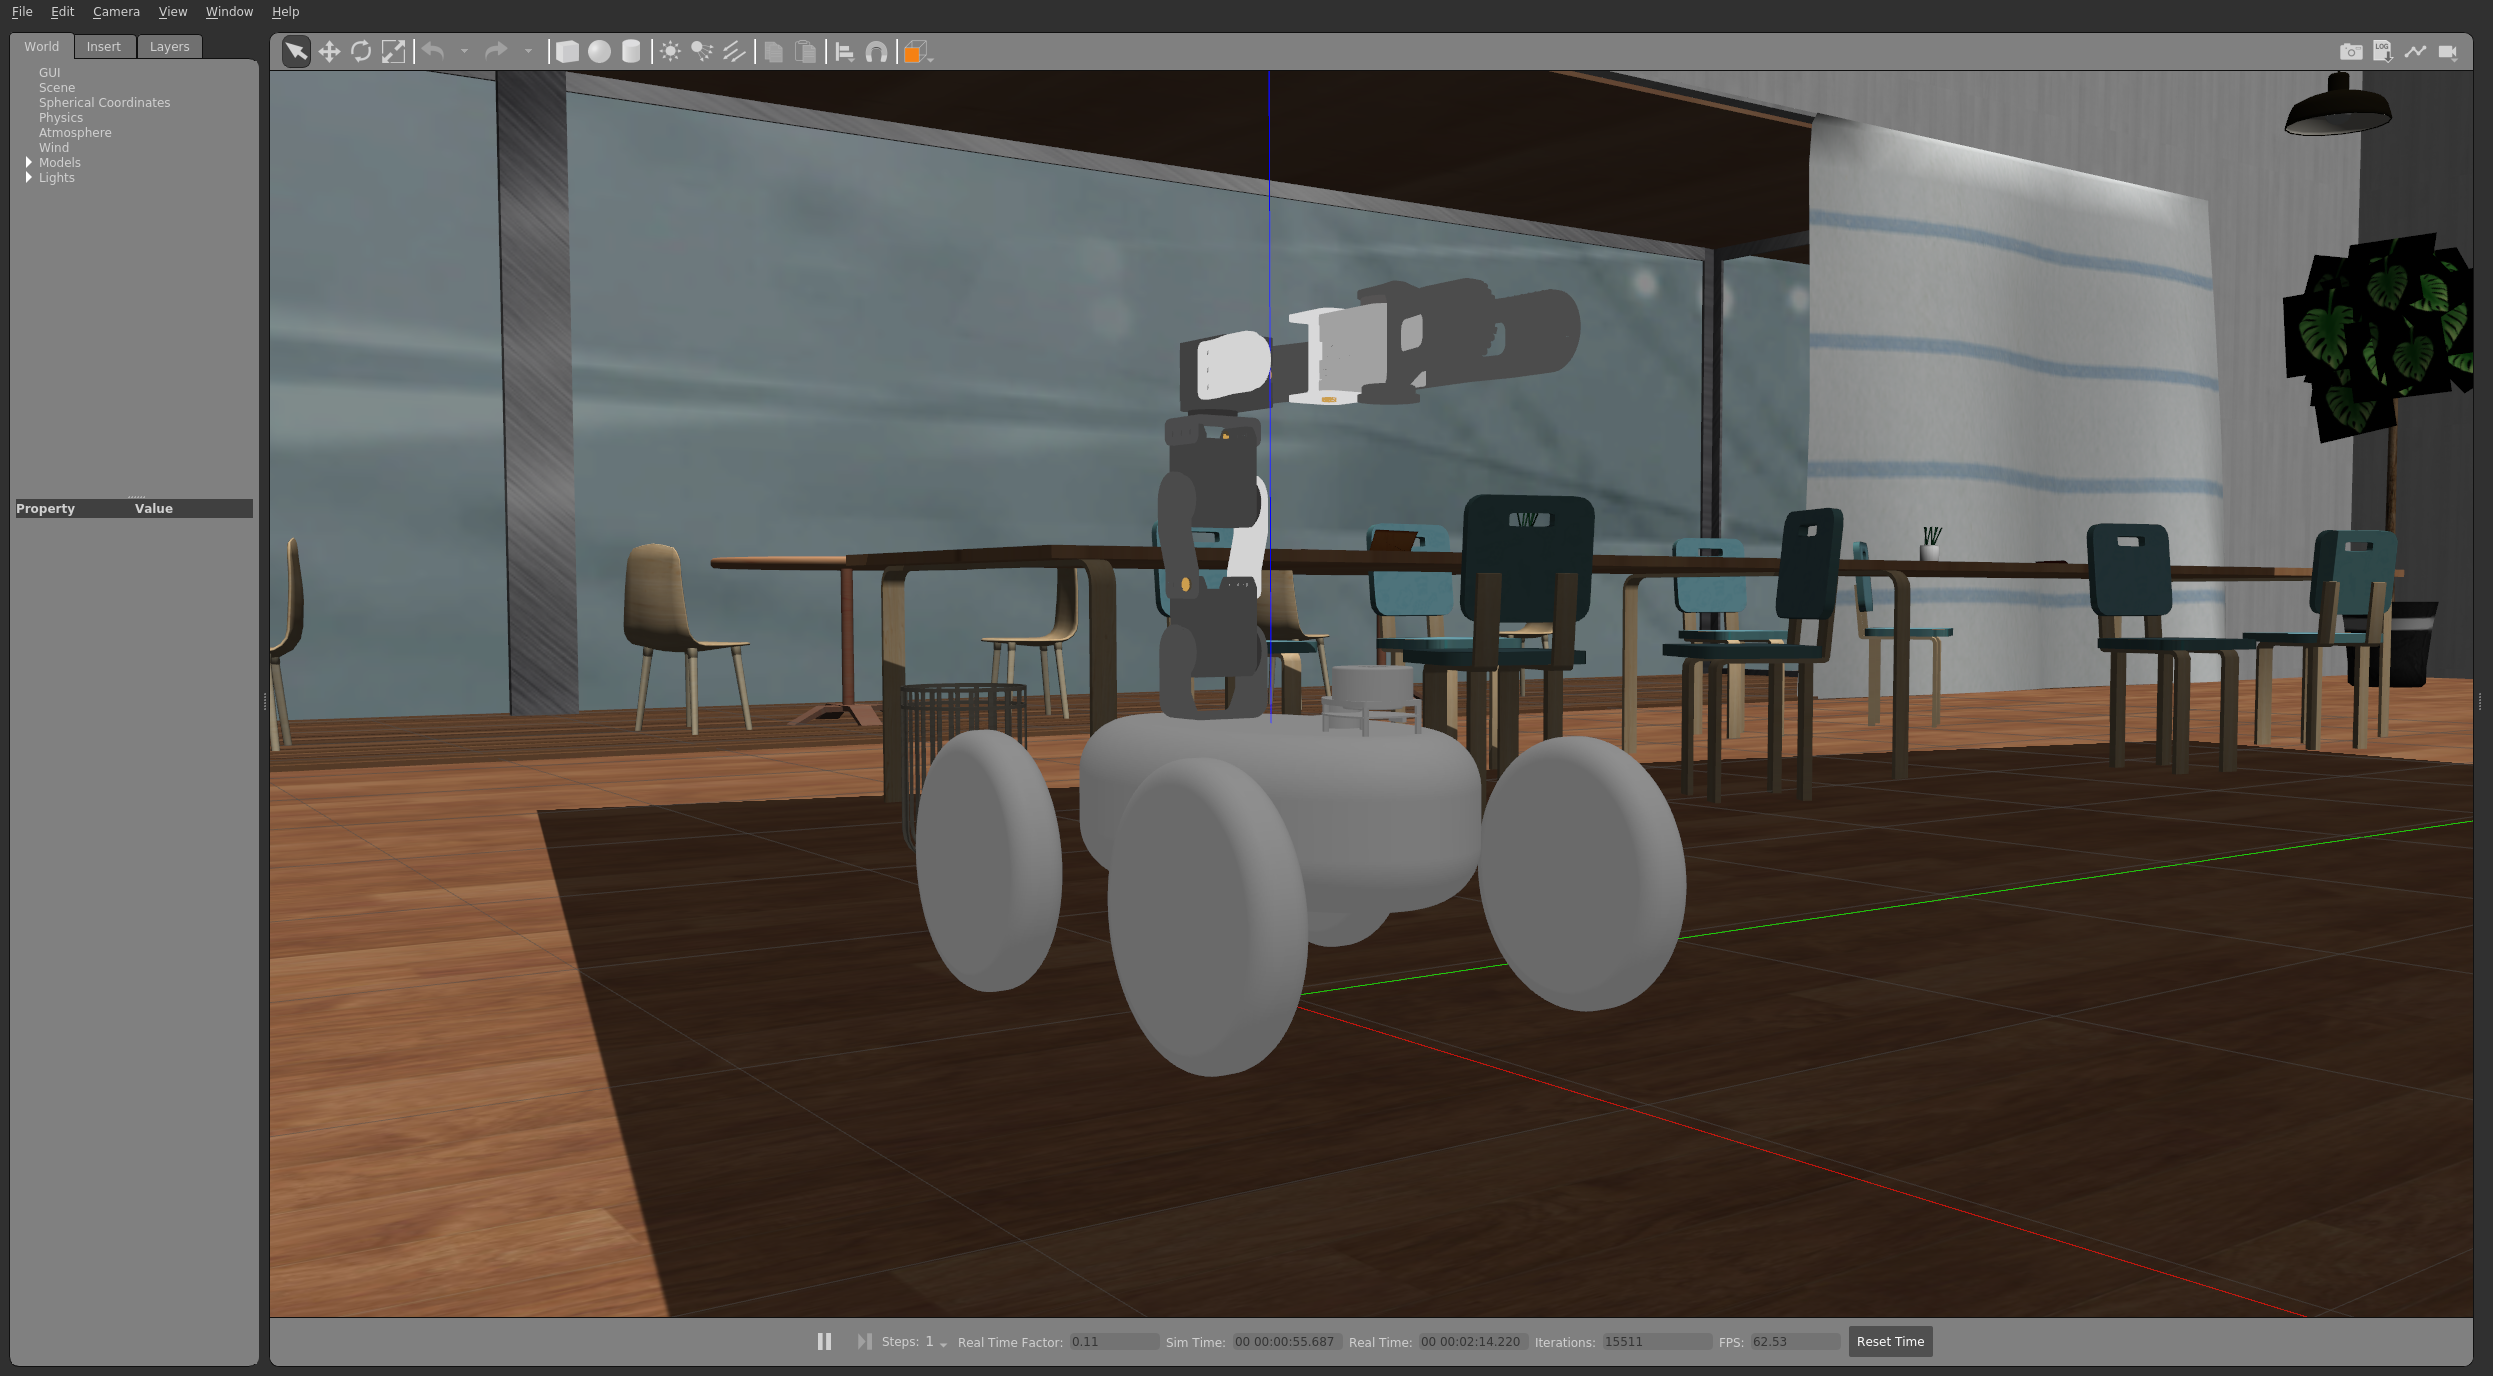
\includegraphics[width=\textwidth]{enlarged-robot.png}
   \caption{Enlarged robot}
   \label{fig:enlarged-robot}
\end{figure}


\subsection{Using beautiful MMD scene}

Figure~\ref{fig:beautiful-scene} is a view of a MMD scene loaded into the Gazebo Classic. It may be that certain physical parameters were not set correctly, even the original tiny robot could not move properly in it.

\begin{figure}[htbp]
   \centering
   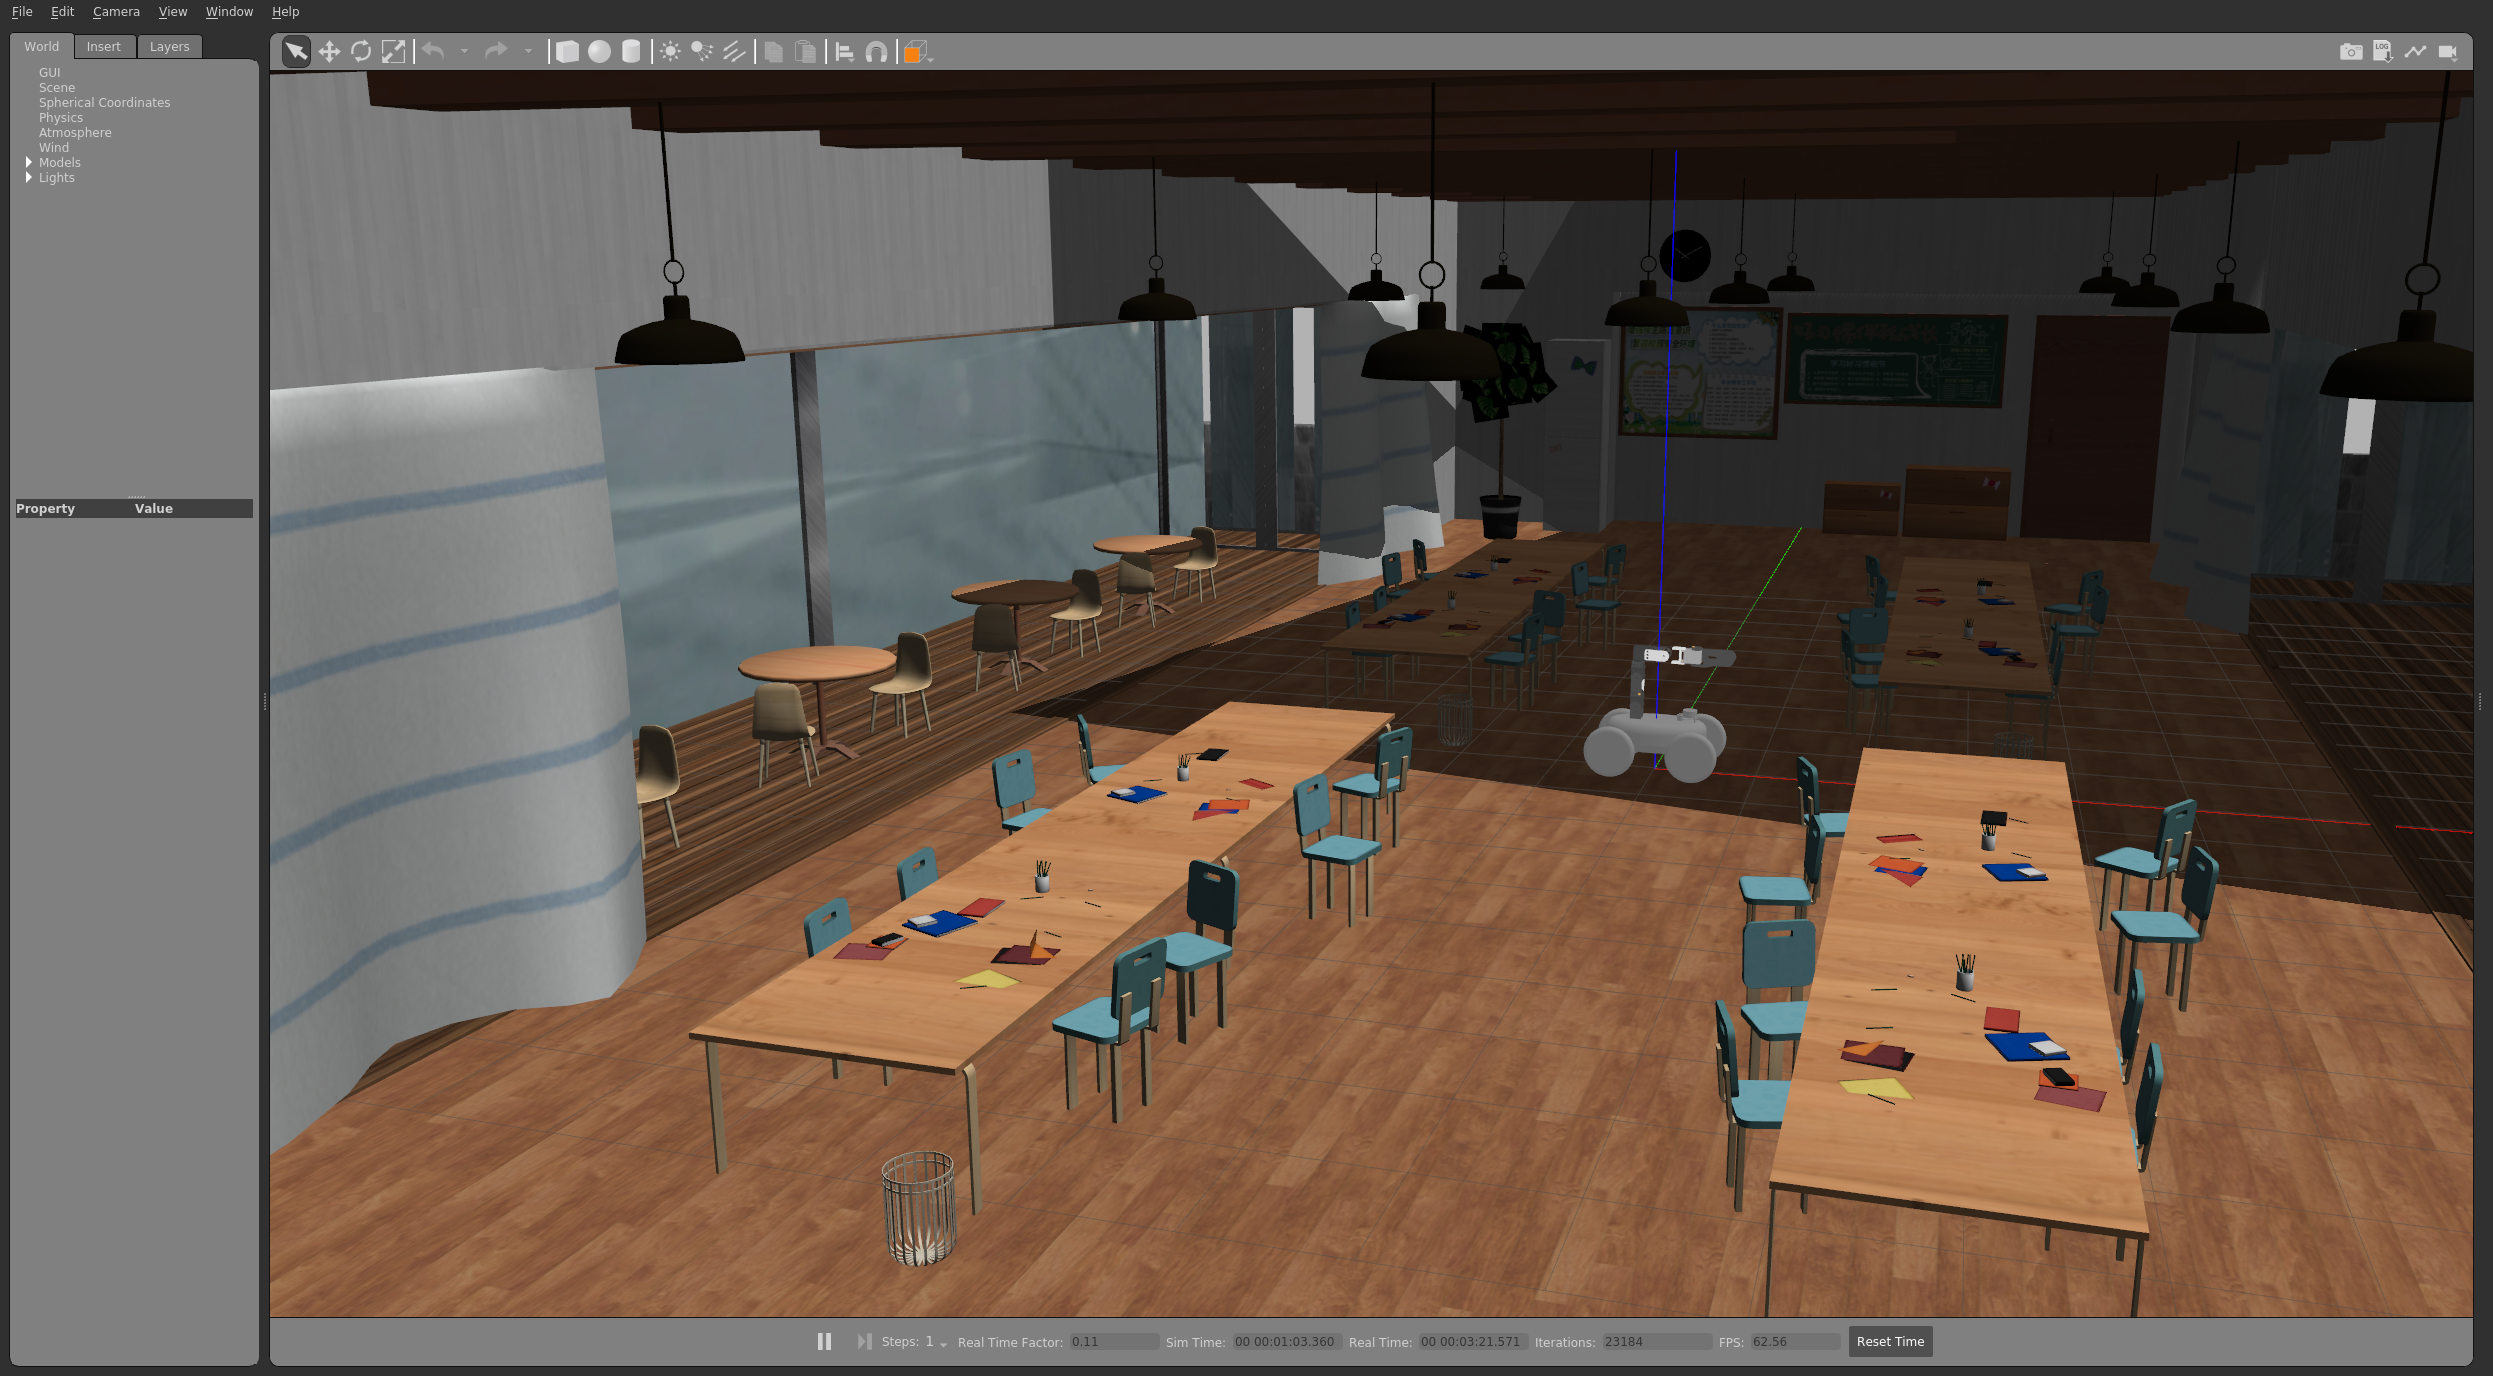
\includegraphics[width=\textwidth]{beautiful-scene.png}
   \caption{A beautiful MMD scene}
   \label{fig:beautiful-scene}
\end{figure}


\subsection{Manually controlling the manipulator by joint state publisher GUI}

When the joint state publisher GUI is enabled, the drive plugin will be disabled and the robot will not be able to move.


\subsection{Including an anime face dataset in training}

I simply do not have time to collate another dataset to train another model.


\subsection{Dynamic obstacles}

Implementing dynamic obstacles such as moving human models enables better testing of navigation capabilities in the simulated testing environment. I have implemented a Python node code to control simple movement of a model. The ultimate goal is to have a human model walking around or dancing in the environment.


\section{Reflections}

I took risks on this assignment. For example, using an anime character model in MMD format, and using an unfamiliar machine learning algorithm for face detection. For the former example, there was no existing work for importing MMDs into Gazebo simulator, but as I was convinced that there must be a way to convert the MMD format into a format that Gazebo can read, I spent bunch of time exploring possible solutions. For the latter example, I didn't realise before I chose to learn how to use YOLOv5 that it requires time-consuming pre-processing of the dataset and long hours of training on cutting-edge high-performance devices. In addition to these two points, I have also searched for better SLAM algorithm and other navigation framework, loaded a much complex indoor environment into the simulator, and enlarge the tiny robot. These explorations and experiments are not directly related to the requirements of the assignment, but are simply my personal interest. I ended up missing the dead line because I took too many risks.

I have encountered many obstacles because I have not mastered the basics. TF is a very common concept in ROS. Many algorithms and components depend on it for their operation. In RViz, for example, the robot model can only be displayed correctly if the right frame is selected. The operation of move\_base package depends on a compliant TF tree: map -> odom -> base\_link -> others. I was stuck on many issues and couldn't solve them because I didn't understand the TF. I should have spent more time learning the basics of ROS.
